\section{Leona Narendra Pahaton}\label{leona-narendra-pahaton}

Tags: NPC Creatore: Lorenzo Luogo: Disharta

\section{\texorpdfstring{\textbf{Leona Narendra
Pahaton}}{Leona Narendra Pahaton}}\label{leona-narendra-pahaton-1}

\begin{center}\rule{0.5\linewidth}{0.5pt}\end{center}

\begin{figure}
\centering
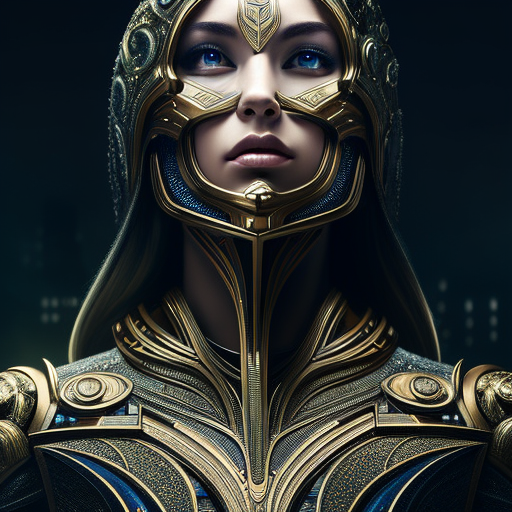
\includegraphics{Principessa_Leona.png}
\caption{Principessa Leona.png}
\end{figure}

Informazioni Generali

Età: 18

Data di nascita: 2005

Luogo di nascita: Goldendor, Disharta

Razza: Umana

Classe:

Alleati:

Nemesi:

Alias:

Professione:

\begin{center}\rule{0.5\linewidth}{0.5pt}\end{center}

\subsection{1. Descrizione Generale}\label{descrizione-generale}

\begin{center}\rule{0.5\linewidth}{0.5pt}\end{center}

\includegraphics{10}\_RITRATTO\_3.png)

La Principessa Leona di Disharta è una figura notevole all'interno del
regno, con una bellezza e grazia che catturano l'attenzione di chiunque
la incontri. ``La sua presenza è maestosa, con capelli dorati che cadono
fluidi sulle spalle e occhi azzurri come il cielo sereno sopra il suo
regno. La sua pelle è chiara, impreziosita da un tocco di rosa sulle
guance, e ha una statura slanciata che riflette l'eleganza della sua
figura regale''. È così che le principesse Dishartane vengono descritte
da sempre, anche se con capelli corti e mori, con gli occhi scuri, basse
e con la pelle color oliva, ovvero come Leona.

\subsection{2. Biografia}\label{biografia}

\begin{center}\rule{0.5\linewidth}{0.5pt}\end{center}

Unica figlia dell'Imperatore Lucius III di Disharta, la vita di Leona è
stata segnata sin dalla nascita da aspettative reali. Crescendo
all'interno delle mura del maestoso palazzo reale, è stata educata nelle
arti della politica e della diplomazia fin dalla giovane età. La sua
infanzia è stata caratterizzata da un profondo senso di dovere nei
confronti del suo popolo e dell'impero. La sua determinazione a non
sottomettersi alle rigide convenzioni dell'impero ha raggiunto l'apice
nel giorno del suo diciottesimo compleanno, quando è fuggita dal palazzo
reale alla vigilia di un matrimonio combinato. Questa scelta coraggiosa
l'ha portata lontano dal suo mondo conosciuto e ha gettato Disharta
nell'incertezza sulla successione. Al momento nessuno sa dove siano
Hakram e Leona, ne se siano ancora vivi.

\subsection{3. Carriera}\label{carriera}

\begin{center}\rule{0.5\linewidth}{0.5pt}\end{center}

Nonostante non abbia mai intrapreso una carriera tradizionale, la sua
fuga ha messo in moto una serie di eventi che influenzano profondamente
e negativamente il destino dell'Impero di Disharta. La sua vita è
diventata una lotta per la sua libertà e indipendenza.

\subsection{4. Personalità}\label{personalituxe0}

\begin{center}\rule{0.5\linewidth}{0.5pt}\end{center}

Leona è cocciuta ma coraggiosa, risoluta nel perseguire i propri
obiettivi, anche a costo di sfidare le convenzioni sociali e politiche.
Amante accanita della lettura e della geografia, trascorre le sue ore
libere immersa in libri che la portano in mondi lontani e sconosciuti. È
un'esperta conoscitrice dei territori di Valtara, anche se le sue
esplorazioni sono limitate all'immaginazione a causa della sua
situazione. Inoltre, il suo cuore è stato rubato da un ladro girovago
che ha incontrato durante una delle sue tante fughe notturne. Il loro
amore è stato rapido ma intenso, e Leona è rimasta incinta di lui.
Questa nuova prospettiva di maternità ha aggiunto ulteriore
determinazione alla sua lotta per la libertà e l'indipendenza, poiché
vuole garantire un futuro migliore per il suo bambino, lontano dagli
obblighi dell'impero Dishartiano.

\subsection{A. Coinvolgimenti in Eventi
Recenti}\label{a.-coinvolgimenti-in-eventi-recenti}

\begin{center}\rule{0.5\linewidth}{0.5pt}\end{center}

\href{Untitled\%20Database\%203437f651bc3346468e1534d3b16d20e1.csv}{Untitled
Database}
